\section{Geographic Location}

First of all, it needs to be clarified, that parts of this attack only works under specific circumstances.
Git commit timestamps are created by taking the current local time of the underlying \ac{os}.
If one wants to show the travel path of a target, the target's \ac{os} needs to automatically adjust the \ac{utc} offset accordingly to the current geographic location of the device.

This feature is available for newer versions of popular \acp{os}, such as \emph{Windows}~\footnote{Ivan Jenic, `Your Time Zone Can Now Switch Automatically in Windows 10', windowsreport.com, https://windowsreport.com/time-zone-automatic-switch-windows-10 (accessed, 24.04.2018)}
and \emph{Mac Os}, but they are not enabled by default.
It is also available for Linux, for instance with the \emph{tzupdate} package~\footnote{`Set the system timezone based on IP geolocation', github.com, https://github.com/cdown/tzupdate (accessed, 24.04.2018)}, but it needs to be manually installed and activated.

\begin{figure}[H]
    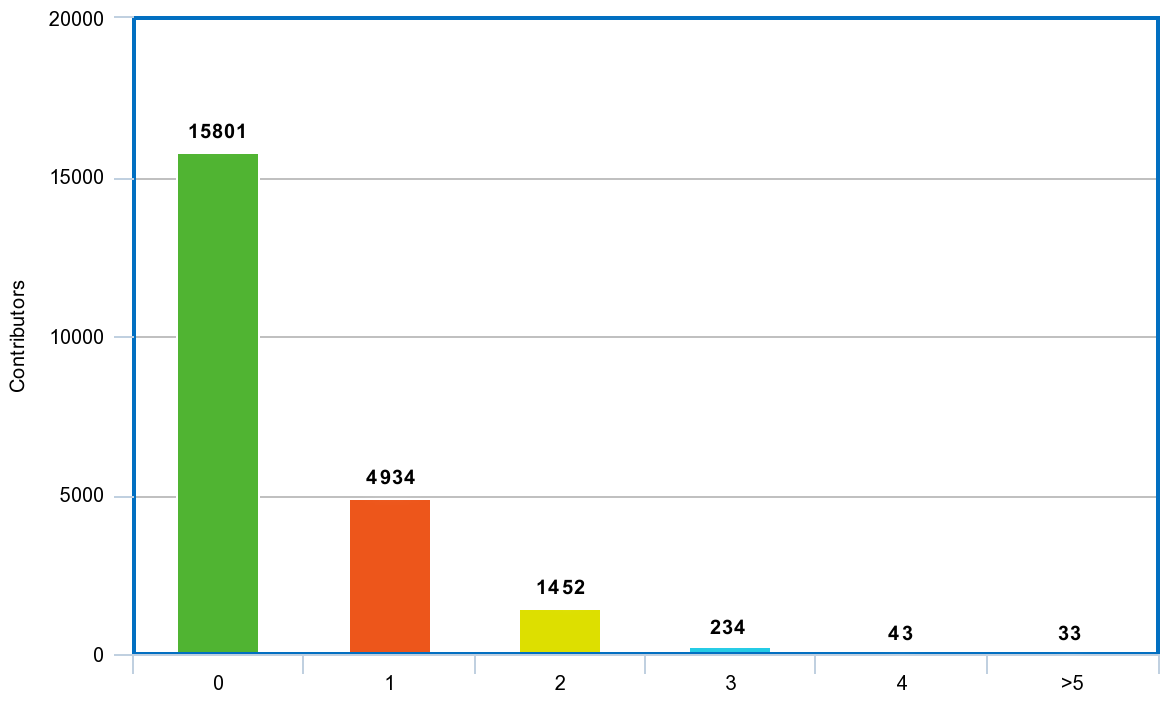
\includegraphics[scale=0.38]{./graphs/analysis/timezone-switch-distribution}
    \centering
    \caption{Distribution of users according to the amount of timezone switches detected by the algorithm.
    The major part of all contributors does not have any detectable timezone changes.}\label{fig:timezone-switch-distribution}
\end{figure}

Figure~\ref{fig:timezone-switch-distribution} shows the number of contributors in relation to the number of detected timezone switches.
On about 70\% of considered contributors, only a single timezone has been detected, looking at the last year.
These 70\% do either not commit if they travel, their \acp{os} do not synchronize the timezone accordingly to their location or they simply did not travel in the last two years.

\begin{figure}[h]
    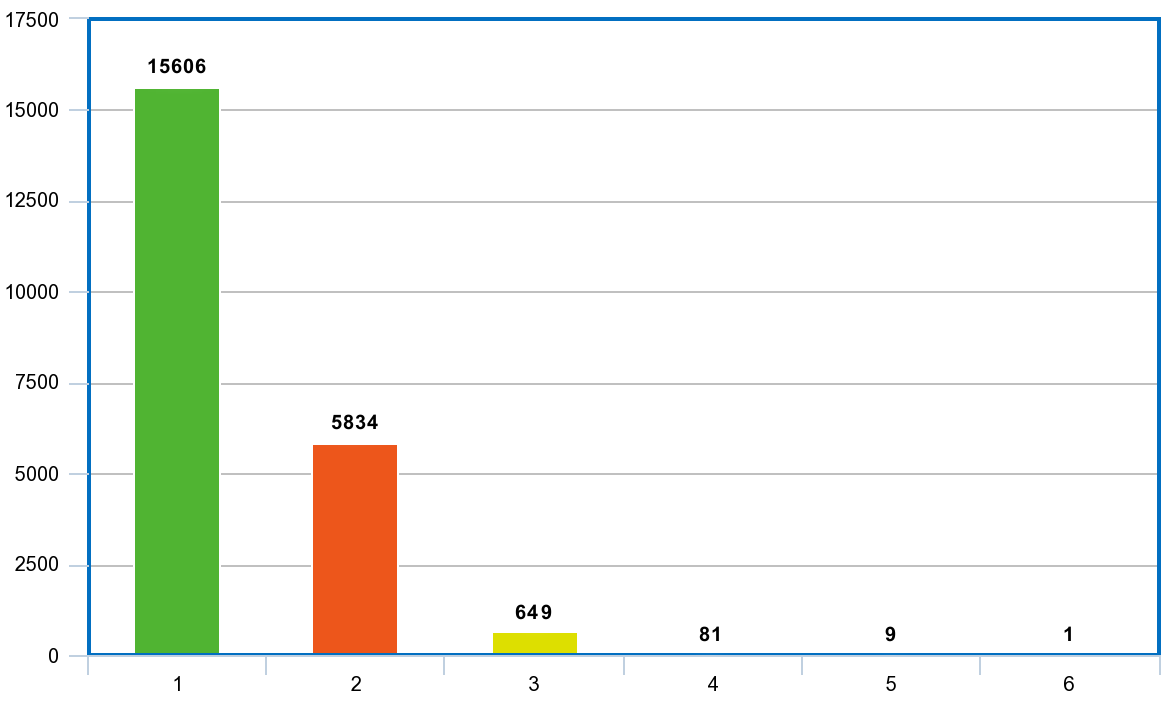
\includegraphics[scale=0.38]{./graphs/analysis/timezone-distribution}
    \centering
    \caption{Distribution of users according to the amount of the different timezones detected by the algorithm.}\label{fig:timezone-distribution}
\end{figure}

In Figure~\ref{fig:author-home-location} the visualized home location analysis of the author can be seen.
Regions marked in dark green are regions in which the contributor is likely to live.
The light green region represents the timezone of the home location.
As you can see in Figure~\ref{fig:author-home-location} the country of French Guiana is also marked as a possible home location.
This problem occurs due to the several conversions between country names and codes, which were necessary as stated in Section~\ref{timezone-implementation}.
This misassignment only happens during the visualization process of the results and thereby does not affect the results of the analysis.

\begin{figure}[h]
    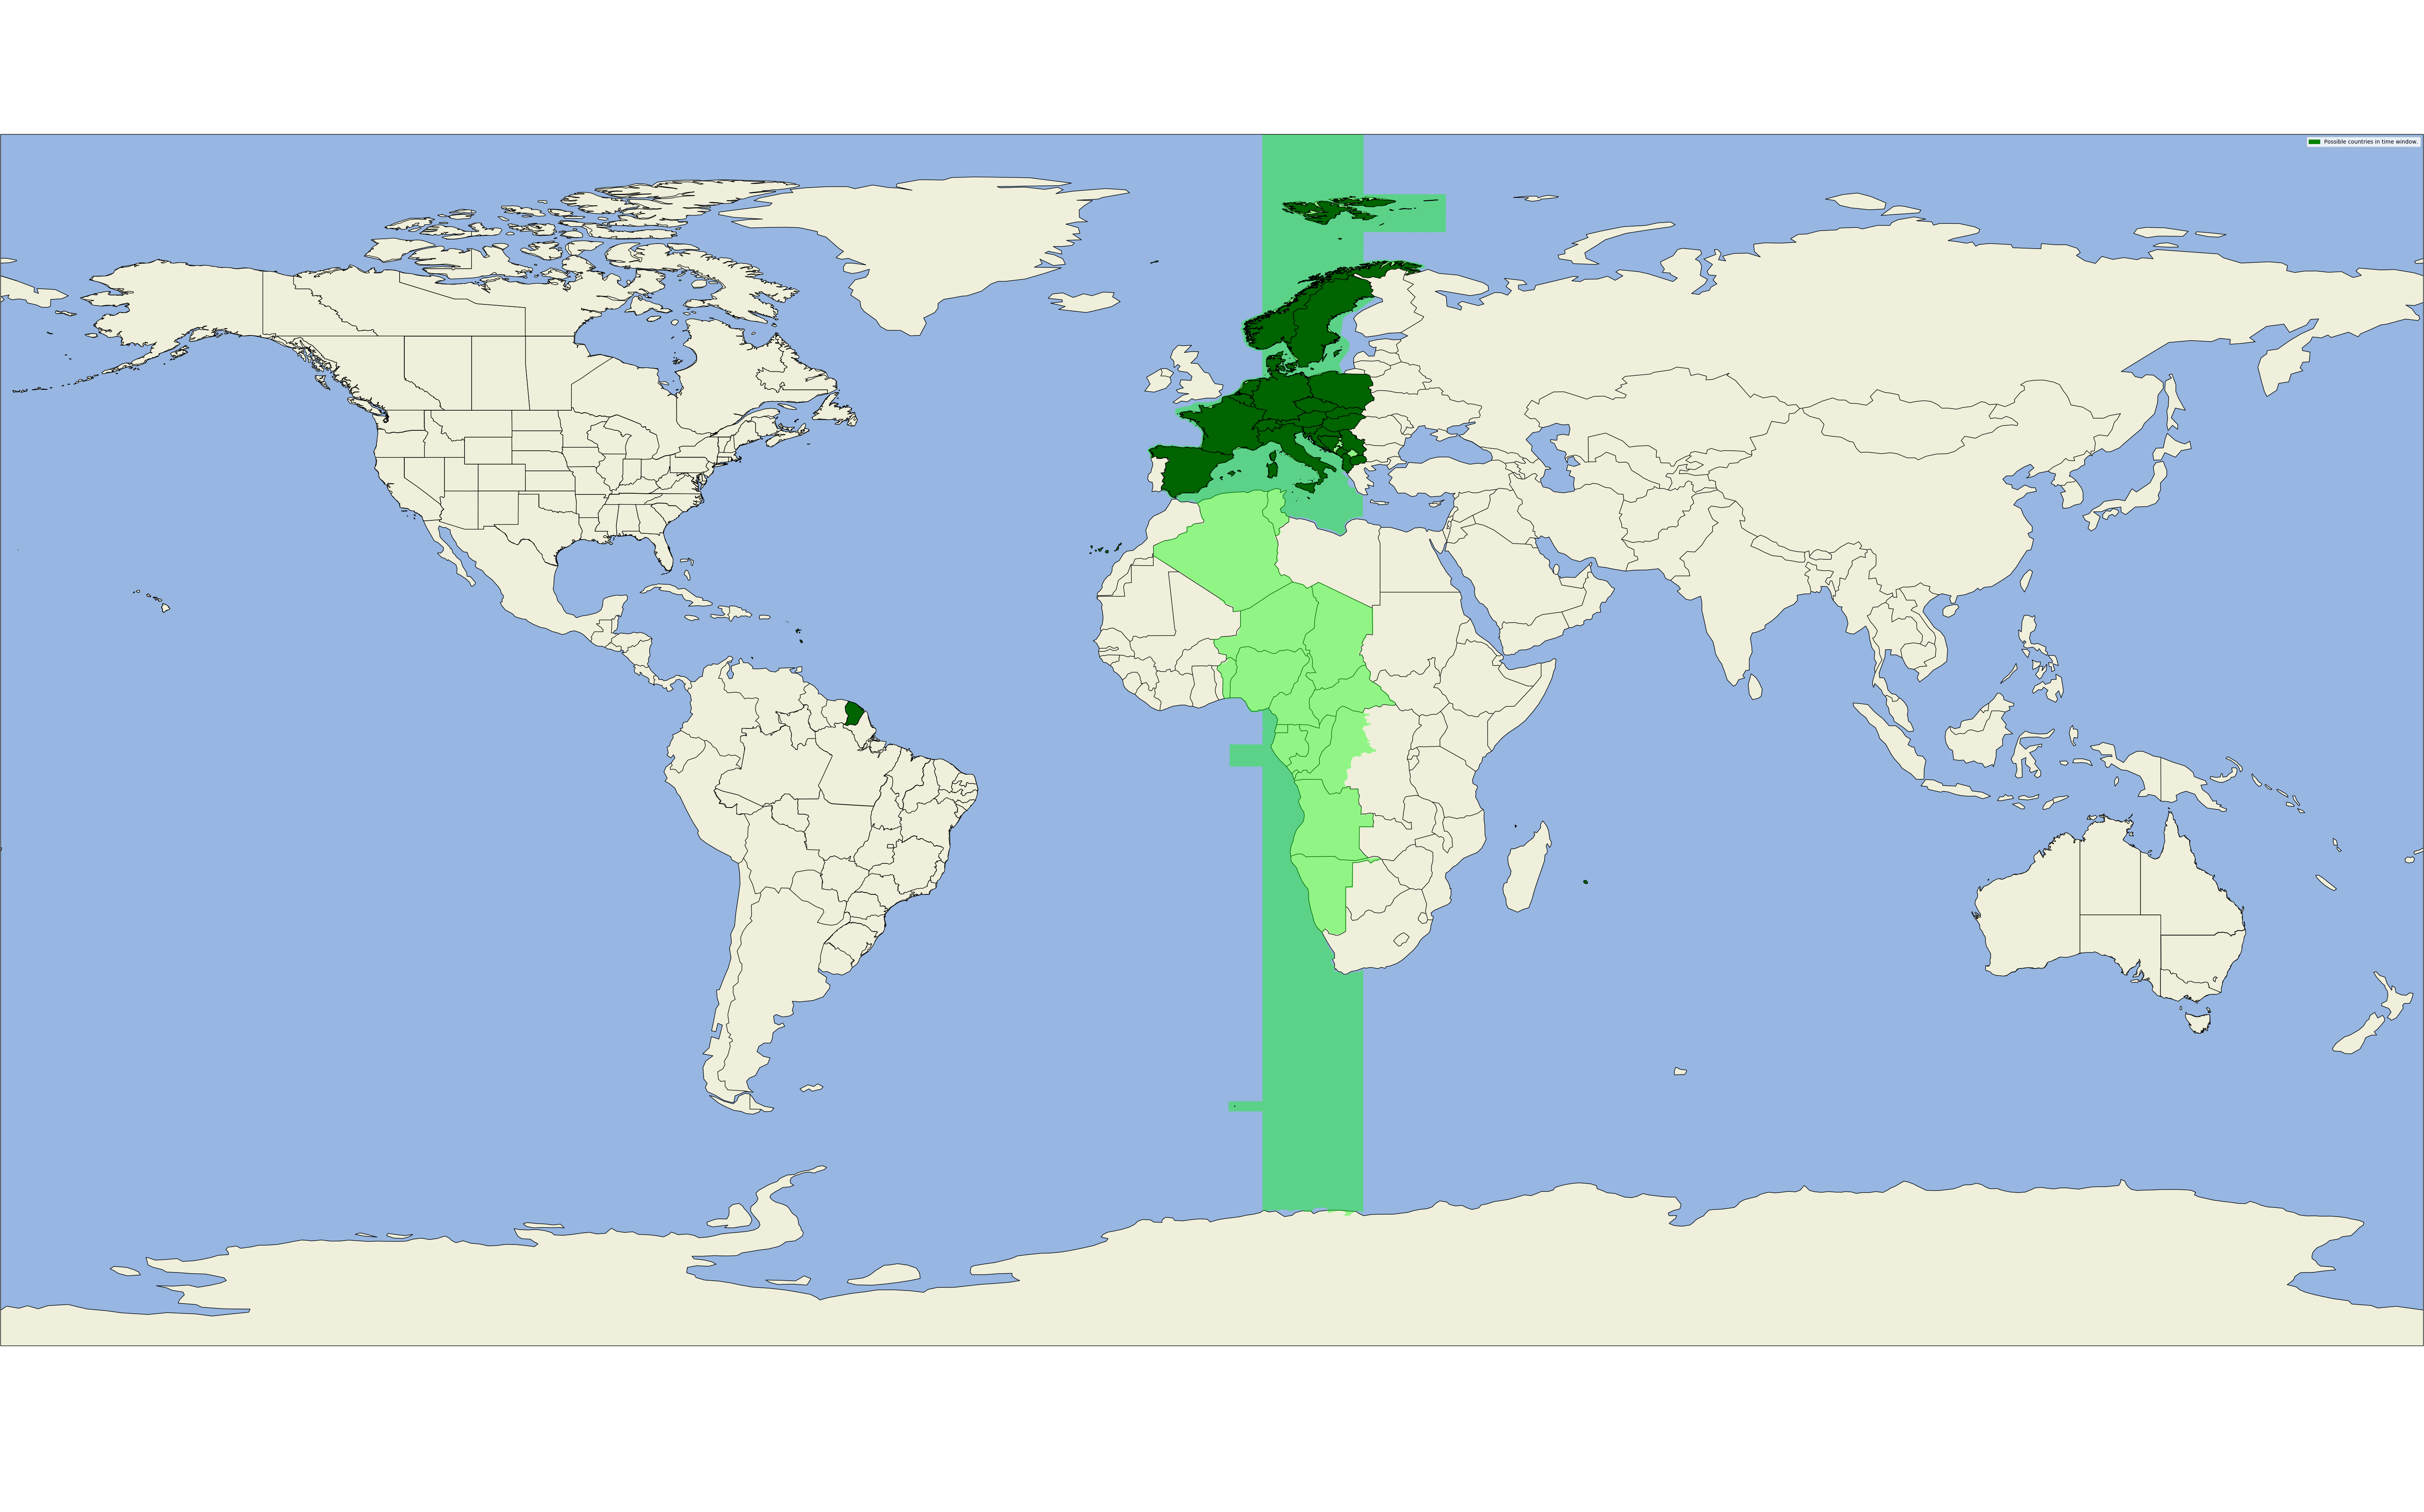
\includegraphics[scale=0.10]{./graphs/analysis/author-home-location}
    \centering
    \caption{The visualized home location analysis of the author.
    The light green indicates the timezone the target is probably in.
    The dark green color shows the remaining countries after considering \ac{dst} switches.}\label{fig:author-home-location}
\end{figure}

To evaluate the overall precision of the geographic location results, the correctness of the determined home locations are checked.
Github allows users to specify a string for their current home location, which is collected during the aggregation process.
Unfortunately, there are no conventions on how this string has to look like.
Initially, I tried to pass these strings to OpenStreetMap, but this resulted in too many wrongly assigned locations.
The data provided by the users was obviously too arbitrary and full of mistakes for the OpenStreetMap \ac{api} to handle.

As a result, I decided to manually choose a subset of locations by looking for distinct identifiers in the location strings.
For instance, every home location of a contributor, that contained \emph{Germany} or \emph{Deutschland} in their location string, should be in the timezone \inlinecode{Europe/Berlin}, which switches between \ac{cet} and \ac{cest}.
I created 14 such rules and was thus able to validate the home location of about 4200 contributors.
The assignment of the contributors home location was correct in about 82\% of the considered contributors.

It needs to be noted, that the accuracy of this result is quite certainly deteriorated by location strings, which contain ambiguous information.
On manual review of the location strings, there were, for instance, strings such as \inlinecode{I love NYC}, which belongs to a developer living in Germany.
The result might also be deteriorated by contributors, which moved to another country in the last year, as we cannot detect those for sure.

It also needs to be noted, that the \ac{iana} database has not always exact mapping for countries to their timezone.
For many countries or states, the current or an old capital city is used.
Some countries do not have an own timezone, for instance, Japan which falls into \inlinecode{Pacific/Palau}.
The \ac{iana} database is the currently best viable approach, but for better results and a more fine-grained resolution, a specific mapping between countries, states and time zones would be necessary.

Nevertheless, an accuracy of 76\% clearly shows, that it is possible to narrow down the location of a contributor to a timezone and even to a subset of countries, see the last column in Table~\ref{home-location-table} for reference, by simply looking at their git commit timestamps.

\begin{landscape}
    \begin{table}[h]
        \centering
        \begin{tabular}{llrrrr}
            \toprule
            Query string & Expected timezone string & Considered & Correct & Timezone strings after DST & Before DST  \\
            \midrule
            & & & & & \\
            San Francisco        & US/Pacific           & 772        & 639     & 12.07   &  18     \\
            NYC, NY, New York    & America/New\_York    & 485        & 366     & 23.60   &  52     \\
            India                & Asia/Colombo         & 148        & 127     & 4       &  4      \\
            UK, United Kingdom   & Europe/London        & 667        & 510     & 13.14   &  22     \\
            France               & Europe/Paris         & 490        & 421     & 31.59   &  40     \\
            New Zealand          & Pacific/Auckland     & 59         & 52      & 4.76    &  9      \\
            Germany, Deutschland & Europe/Berlin        & 976        & 846     & 31.48   &  38     \\
            Poland               & Europe/Warsaw        & 180        & 154     & 31.56   &  40     \\
            Italy                & Europe/Rome          & 130        & 112     & 31.39   &  41     \\
            Tokyo                & Pacific/Palau        & 61         & 48      & 8.51    &  12     \\
            Spain                & Europe/Madrid        & 129        & 116     & 32.83   &  40     \\
            Los Angeles          & America/Los\_Angeles & 86         & 76      & 12.24   &  18     \\
            Adelaide             & Australia/Adelaide   & 2          & 2       & 4.00    &  4      \\
            Mexico               & Mexico/General       & 13         & 7       & 11.62   &  39     \\
            \bottomrule
        \end{tabular}
        \caption{Results of the home location evaluation.
        The first column shows the comma separated strings by which contributors are selected depending on their location.
        The second column is the timezone that is expected to be in the remaining home location timezone string set.
        }\label{home-location-table}
    \end{table}
\end{landscape}
